\chapter{System Design and Architecture}
\label{chapter:architecture}

The design and architecture of a system are crucial elements that profoundly impact its functionality, efficiency, and scalability. 
\\
This chapter outlines the foundational components of the proposed proof-of-concept for the SPLASH system, illustrating how various elements interact to form a cohesive and effective solution for beach safety management. 
\\ 
It explores several essential diagrams that depict the system's architecture and operational framework. Each diagram serves a distinct purpose in visualizing different aspects of the system, enhancing our understanding of its structure and functionality. By systematically analysing these diagrams, we aim to develop a comprehensive understanding of \ac{splash}'s design principles and operational capabilities and lay the groundwork for further exploration into its implementation and potential impact on beach safety management.
\\

\newpage
\section{Context Diagram}
\label{section:context_diag}
This diagram \ref{fig:context_diag} offers a comprehensive, high-level overview of the system's interactions with external entities, highlighting key interfaces and relationships.

\begin{figure}[H]
      \centering
      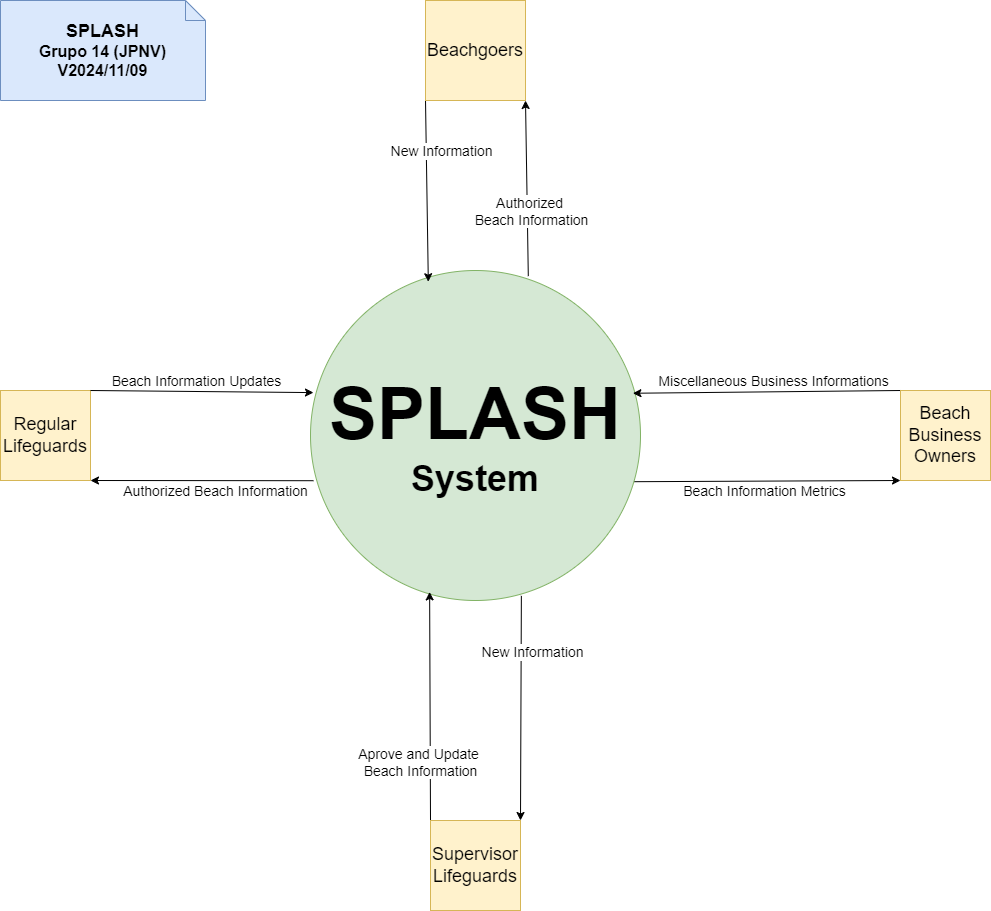
\includegraphics[width=16cm]{figs/context_diagram.png}
      \caption{SPLASH: System Context Diagram. For a more detailed view: \url{https://github.com/JoaoPNVieira/PECI-24-25/tree/main/Milestones}}
      \label{fig:context_diag}
\end{figure}

\newpage
\section{High-Level Architecture Diagram}
\label{section:high_level_diag}
This section presents a diagram \ref{fig:diag_high_level.png} that serves as an architectural blueprint of the system, showcasing its major components and their relationships, which is crucial for understanding the overall structure.

\begin{figure}[H]
      \centering
      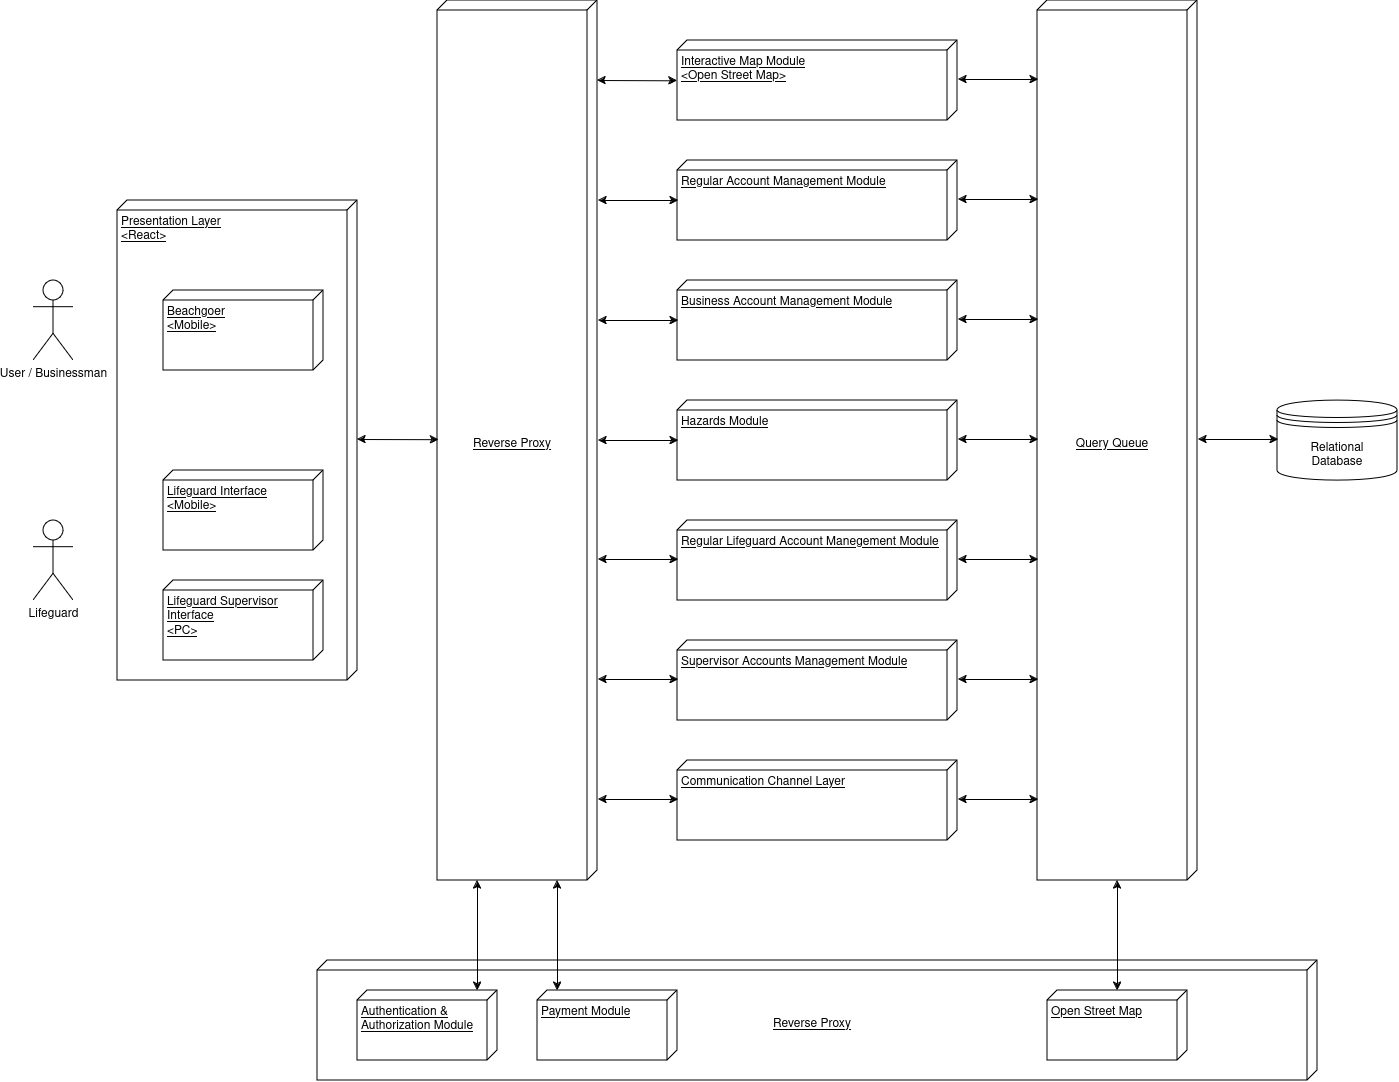
\includegraphics[width=16cm]{figs/diag_high_level.png}
      \caption{SPLASH: System High-Level Architecture Diagram. For a more detailed view: \url{https://github.com/JoaoPNVieira/PECI-24-25/tree/main/Milestones}}
      \label{fig:high_level_diag}
\end{figure}

\newpage
\section{Use-Case Diagram}
Here \ref{fig:use_case_diagram}, we will define the various user interactions with the system, identifying key functionalities that serves to both beachgoers and lifeguards organizations. 

\begin{figure}[H]
      \centering
      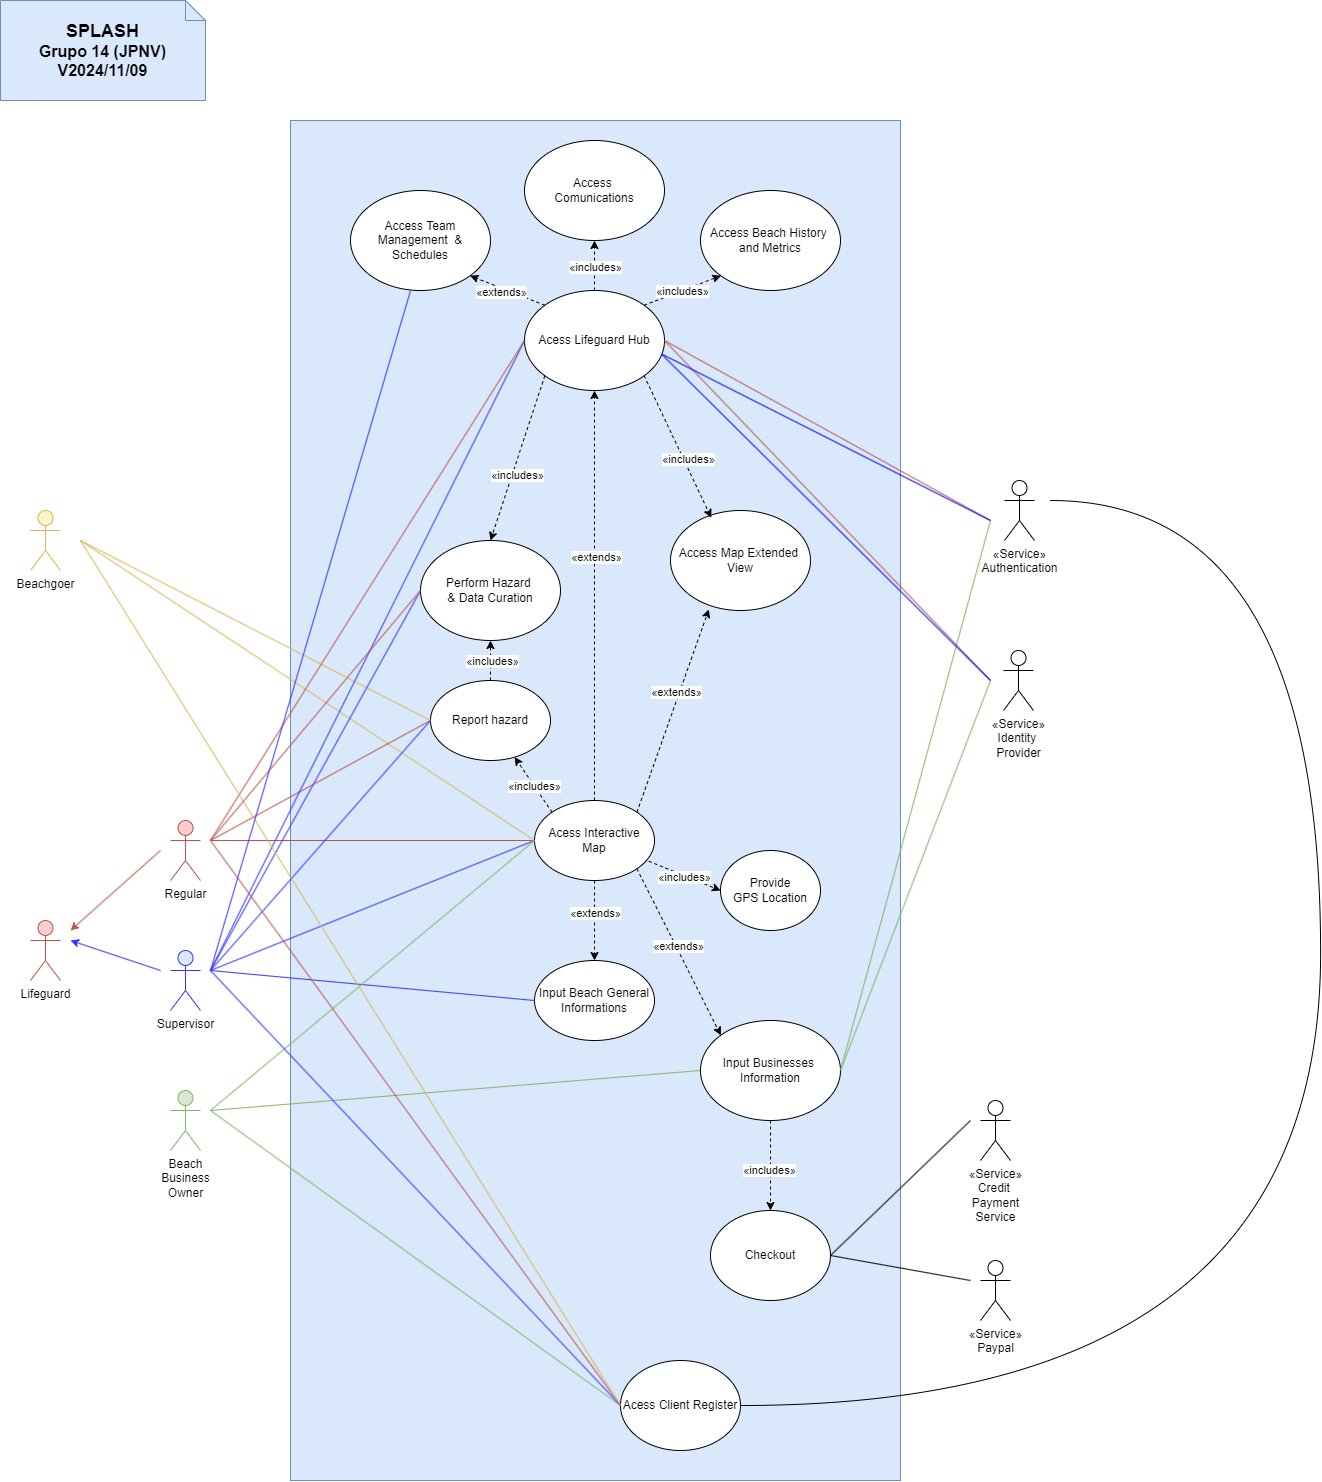
\includegraphics[width=16cm]{figs/use_case_diagram.png}
      \caption{SPLASH: System Use-Case Diagram. For a more detailed view: \url{https://github.com/JoaoPNVieira/PECI-24-25/tree/main/Milestones}}
      \label{fig:use_case_diagram}
\end{figure}

\newpage
\section{Components Diagram}
This diagram \ref{fig:componets} delves into the individual components of the system, illustrating how they work together to deliver the desired outcome.

\begin{figure}[H]
      \centering
      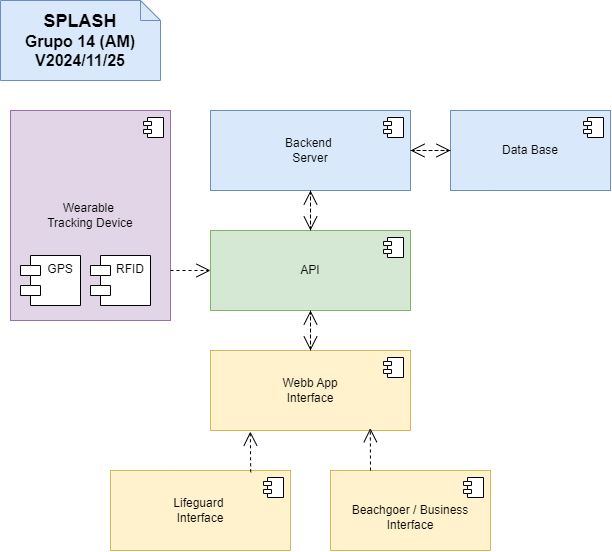
\includegraphics[width=16cm]{figs/componets.png}
      \caption{SPLASH: System Components Diagram. For a more detailed view: \url{https://github.com/JoaoPNVieira/PECI-24-25/tree/main/Milestones}}
      \label{fig:componets}
\end{figure}

\newpage
\section{Data Flow Diagram}
In this section the diagram \ref{fig:data_flow} visualizes the flow of data within the system, providing insights into how information is processed and utilized to enhance decision-making.

\begin{figure}[H]
      \centering
      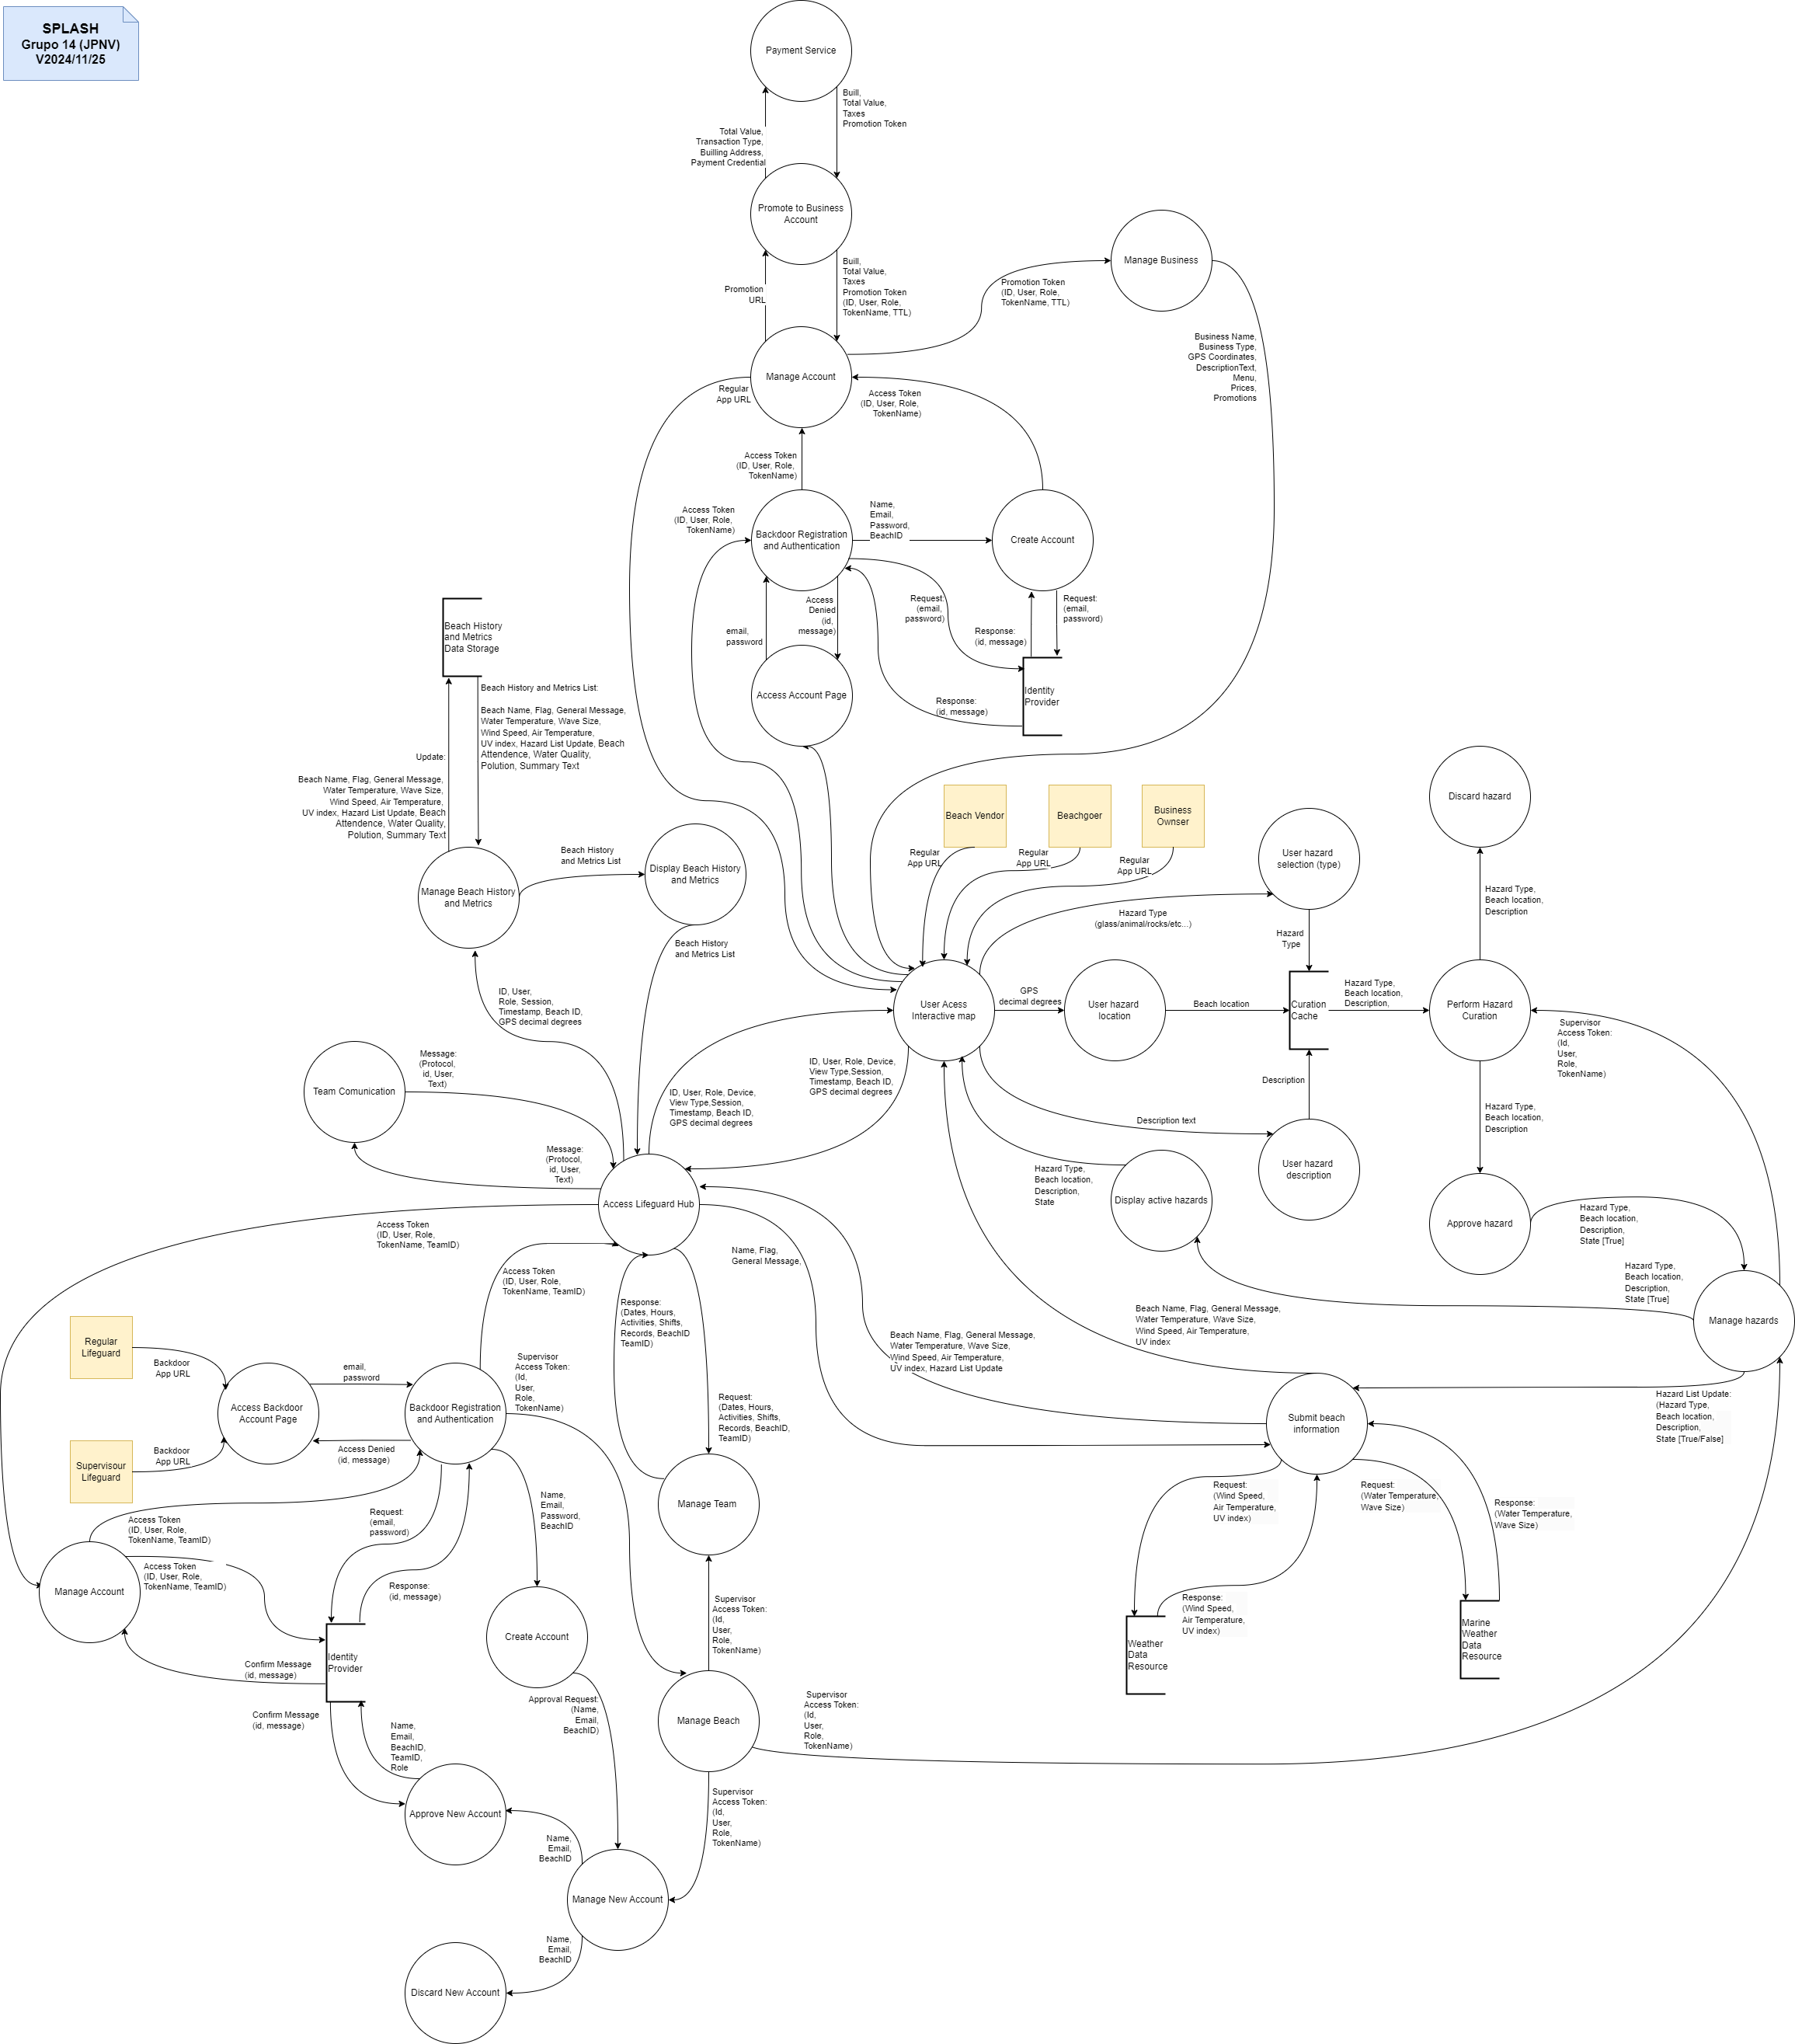
\includegraphics[width=16cm]{figs/data_flow.png}
      \caption{SPLASH: System Data Flow Diagram. For a more detailed view: \url{https://github.com/JoaoPNVieira/PECI-24-25/tree/main/Milestones}}
      \label{fig:data_flow}
\end{figure}

\newpage
\section{Deployment Diagram}
The following diagram \ref{fig:deployment} will outline how the system will be deployed in real-world scenarios, detailing the physical arrangement of hardware and software components.

\begin{figure}[H]
      \centering
      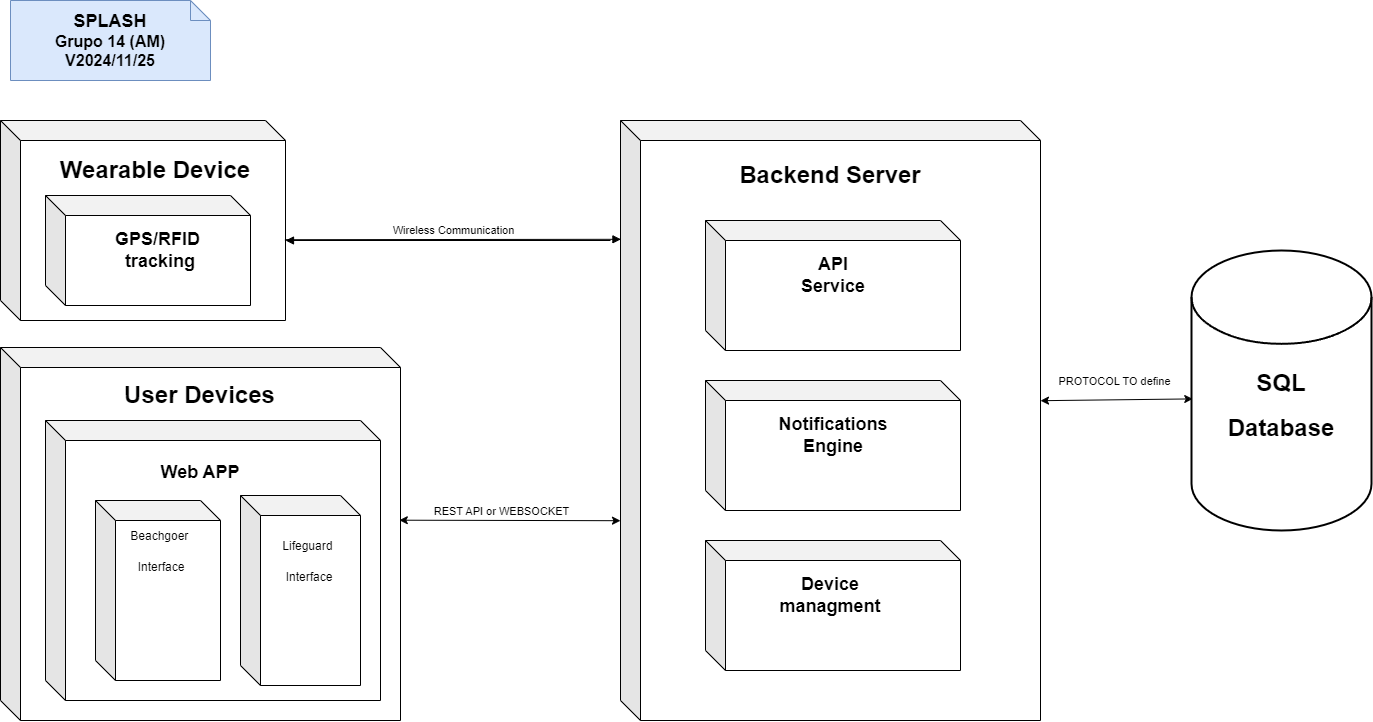
\includegraphics[width=16cm]{figs/deployment.png}
      \caption{SPLASH: System Deployment Diagram. For a more detailed view: \url{https://github.com/JoaoPNVieira/PECI-24-25/tree/main/Milestones}}
      \label{fig:deployment}
\end{figure}

\newpage
\section{General Architecture Diagram}
Finally, this diagram \ref{fig:general_architecture} encapsulates all architectural elements into a single view, summarizing how SPLASH operates as a unified system.

\begin{figure}[H]
      \centering
      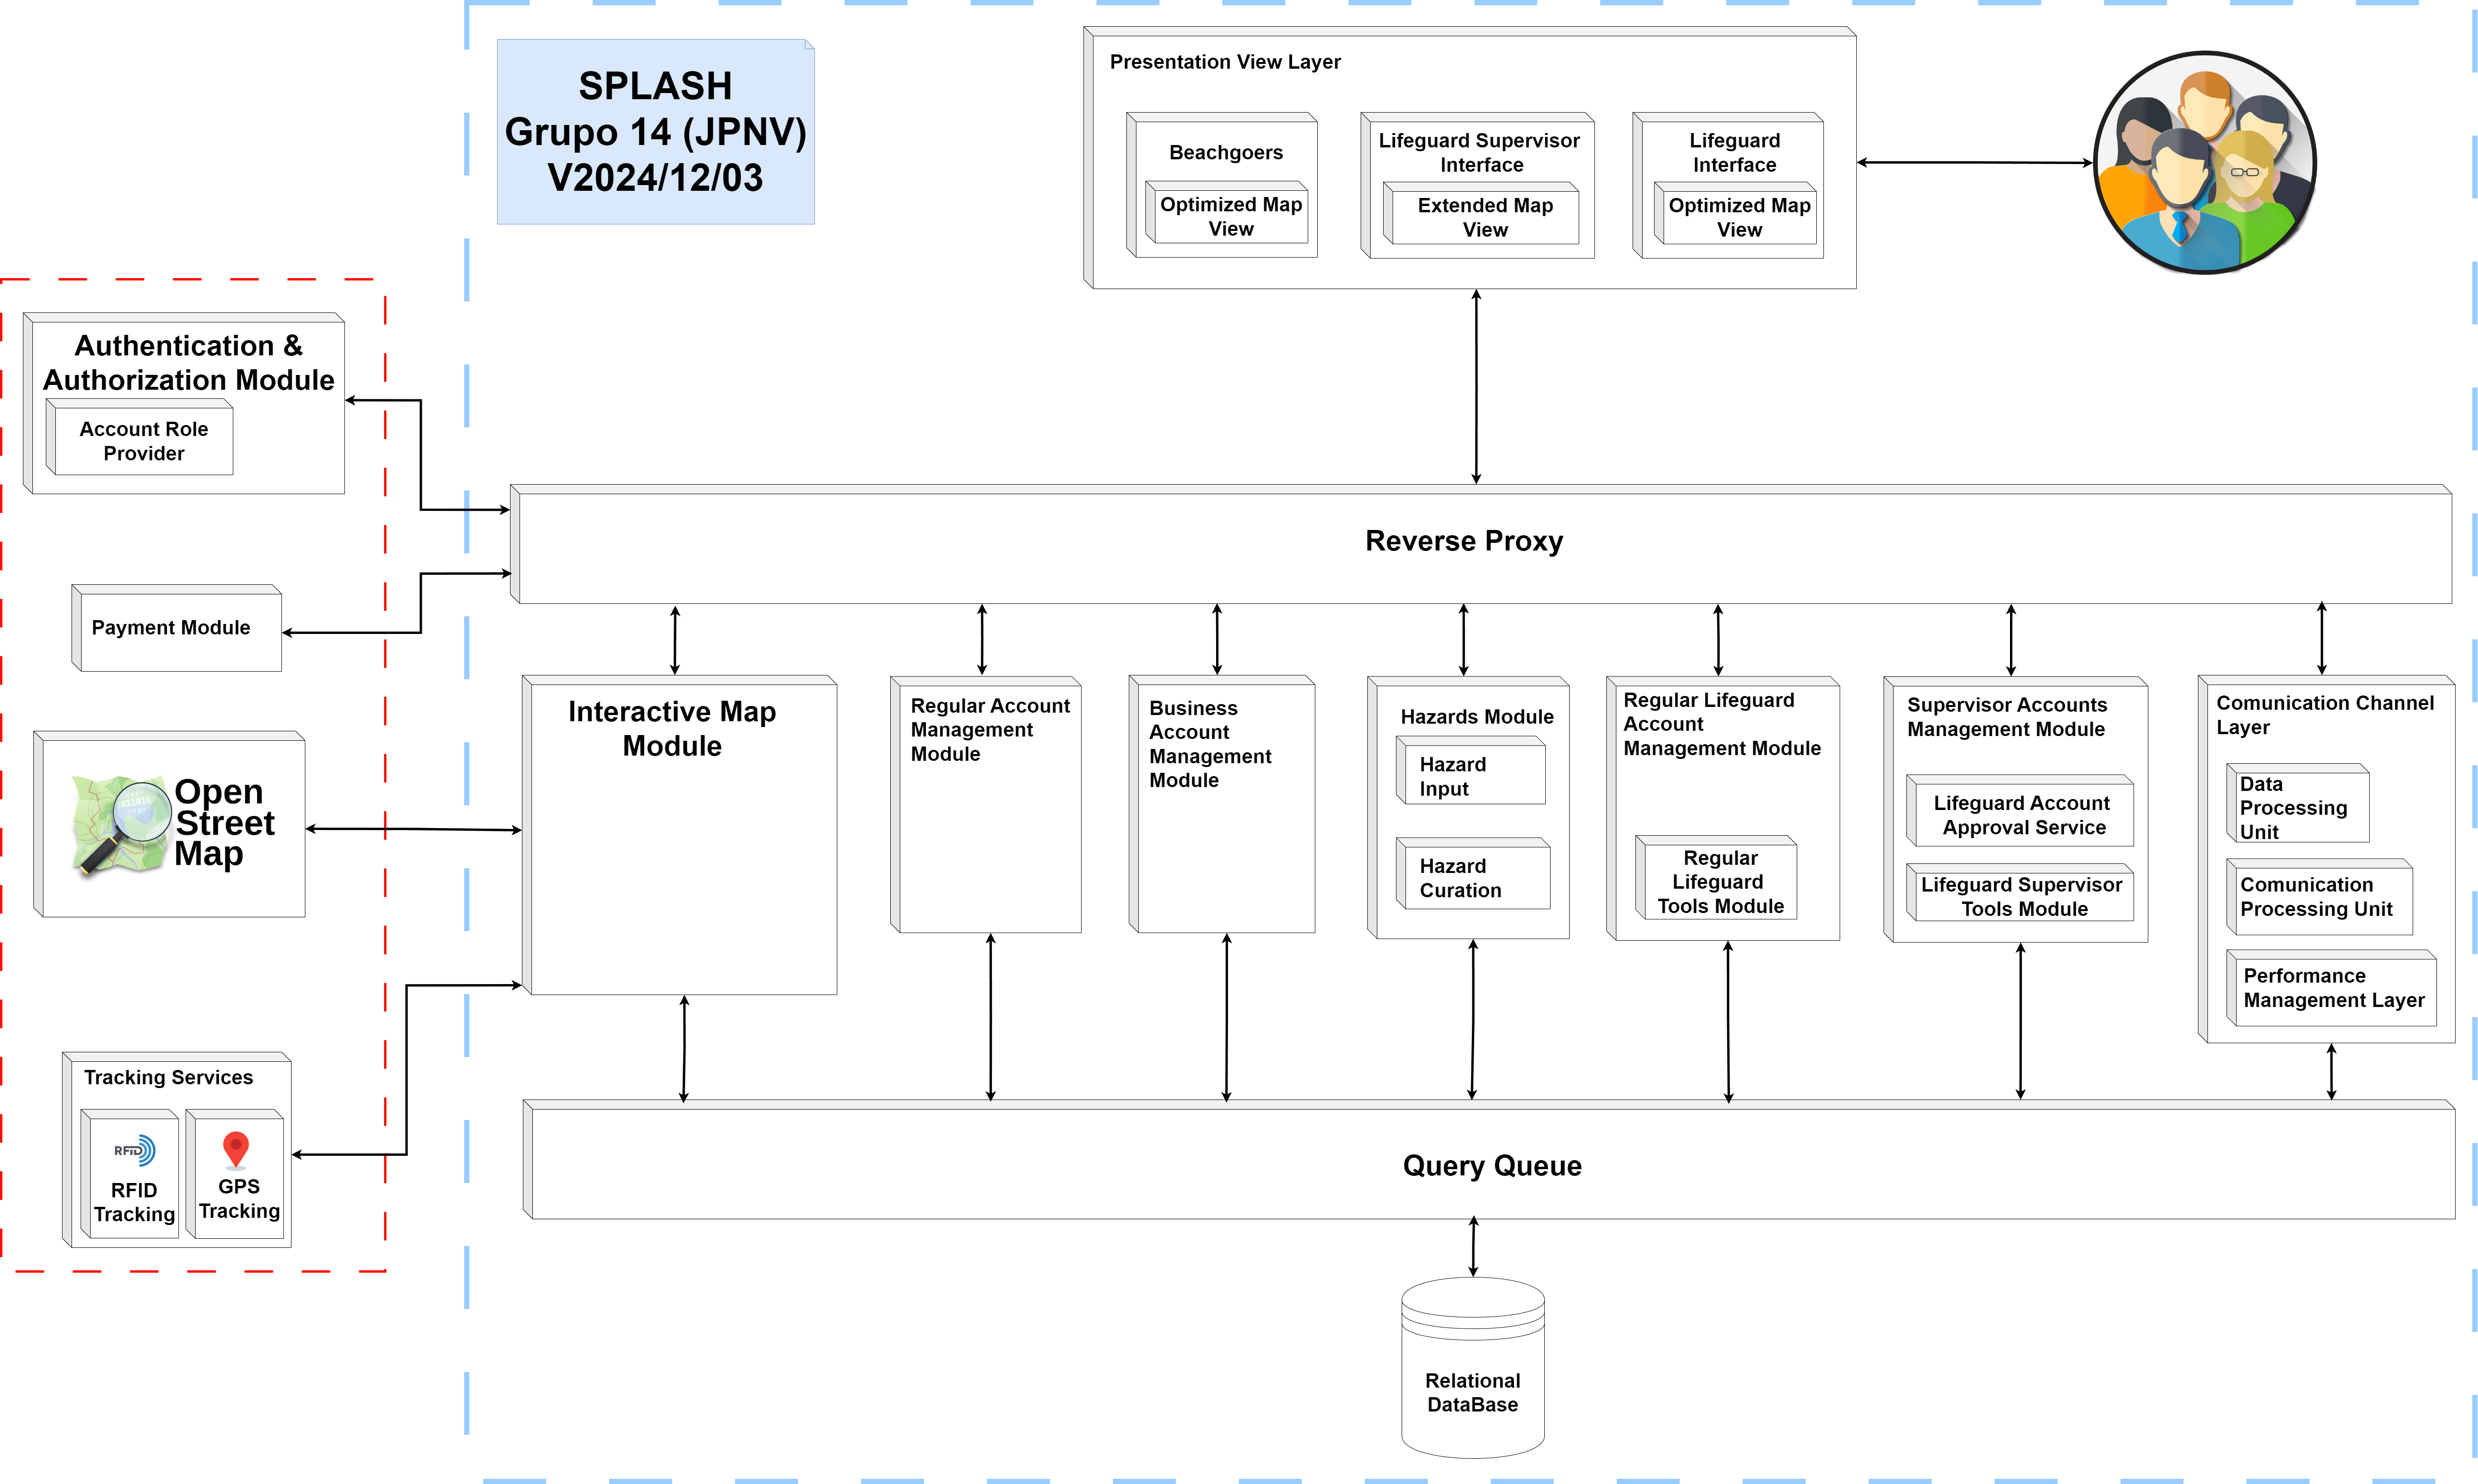
\includegraphics[width=16cm]{figs/general_architecture.png}
      \caption{SPLASH: System General Architecture Diagram. For a more detailed view: \url{https://github.com/JoaoPNVieira/PECI-24-25/tree/main/Milestones}}
      \label{fig:general_architecture}
\end{figure}

\section{Candidate Technologies}
\label{section:candidate_tech}
%
In this project, after developing various diagrams and engaging in multiple discussions, it was decided to create a web app using React and implement a relational database. Simultaneously, it was determined that the wearables would include GPS functionality and identification through RFID technology.

The decision to use React for the web app was based on its flexibility, component-based structure, and ability to build highly interactive user interfaces. 

A relational database was chosen to efficiently manage structured data and relationships, ensuring scalability and reliability.

The inclusion of GPS in the wearables allows real-time location tracking, crucial for features such as safety monitoring and providing alerts about hazardous zones. 

RFID technology ensures quick and secure identification of users, enabling seamless integration with other systems and functionalities, such as linking individual profiles to specific devices or locations.

This architecture ensures that the solution is robust, user-friendly, and capable of addressing the key objectives of the project while leveraging modern technologies to enhance safety and usability

\section{Database Design}
\label{section:dbdesign}

As mentioned earlier, the project will utilize a relational database connected to a \ac{dbms}. Below is the initial draft following our requirements analysis:

\subsection{Entity Relationship Diagram}
\label{subsection:DER}

    \begin{figure}[H]
          \centering
          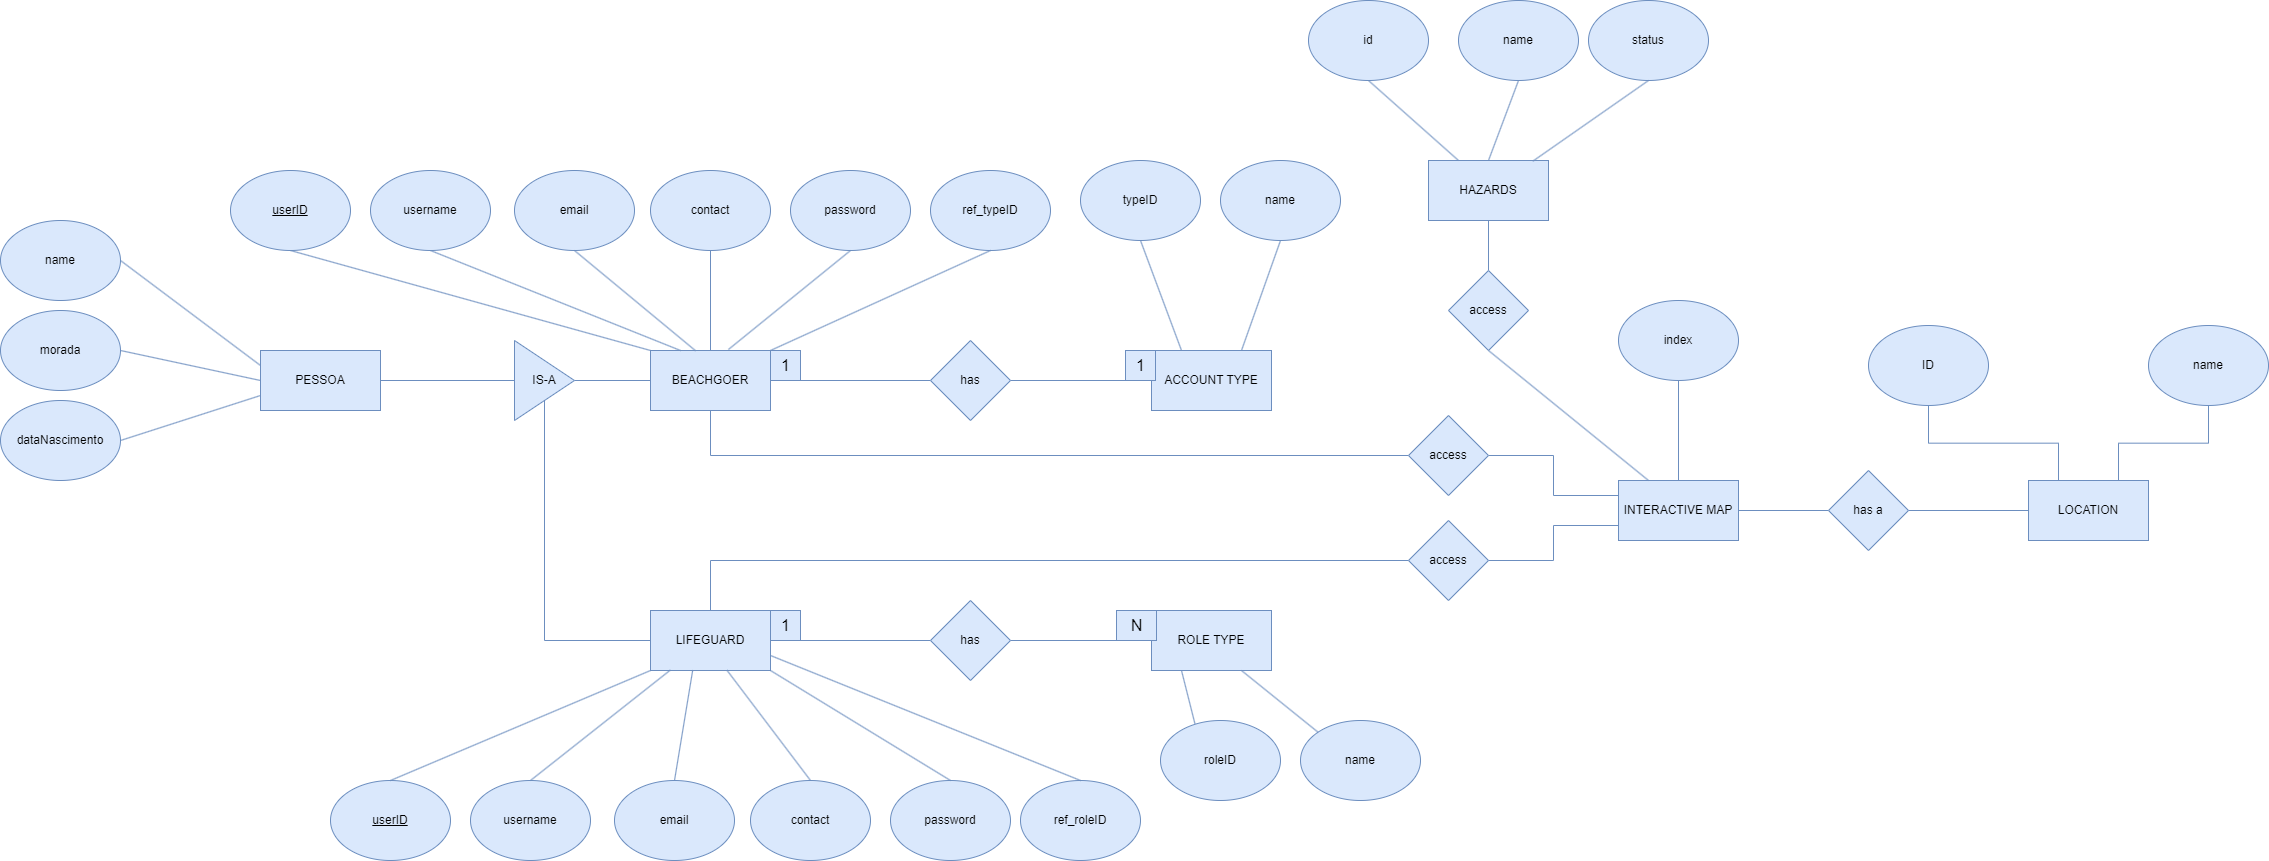
\includegraphics[width=16cm]{figs/DER.png}
          \caption{SPLASH: Entity Relationship Diagram. For a more detailed view: \url{https://github.com/JoaoPNVieira/PECI-24-25/tree/main/Milestones}}
          \label{fig:DER}
    \end{figure}


    